\hypertarget{Utils_8h}{
\section{Utils.h File Reference}
\label{Utils_8h}\index{Utils.h@{Utils.h}}
}


This graph shows which files directly or indirectly include this file:\nopagebreak
\begin{figure}[H]
\begin{center}
\leavevmode
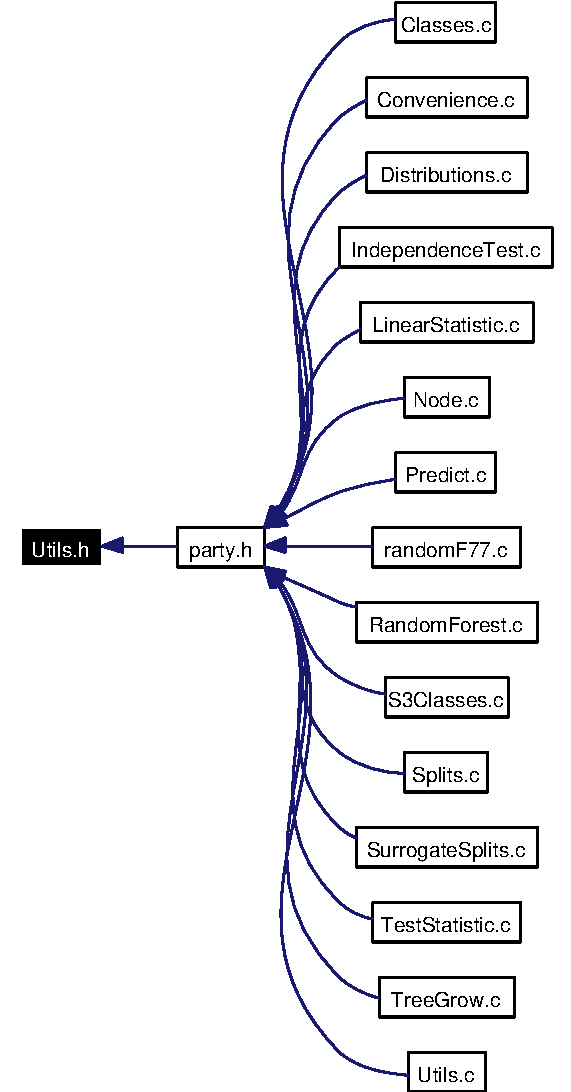
\includegraphics[width=420pt]{Utils_8h__dep__incl}
\end{center}
\end{figure}
\subsection*{Functions}
\begin{CompactItemize}
\item 
void \hyperlink{Utils_8h_12e882779ecd0445c3a0dd9ac85dfeee}{C\_\-kronecker} (const double $\ast$A, const int m, const int n, const double $\ast$B, const int r, const int s, double $\ast$ans)
\item 
SEXP \hyperlink{Utils_8h_572286b2fd0bd9993473cfd0c6b165c0}{La\_\-svd} (SEXP jobu, SEXP jobv, SEXP x, SEXP s, SEXP u, SEXP v, SEXP method)
\item 
void \hyperlink{Utils_8h_f7c710920d1496d23fdabad9b1d0e18c}{C\_\-SampleNoReplace} (int $\ast$x, int m, int k, int $\ast$ans)
\item 
void \hyperlink{Utils_8h_c0d5c2fe971923d7a1b1869dffabddb1}{C\_\-MPinv} (SEXP x, double tol, SEXP svdmem, SEXP ans)
\item 
double \hyperlink{Utils_8h_5b306a6923d1155e6ce877cf6fa12a42}{C\_\-max} (const double $\ast$x, const int n)
\item 
void \hyperlink{Utils_8h_a5479e1fef3da77537e06730826379e1}{C\_\-abs} (double $\ast$x, int n)
\item 
void \hyperlink{Utils_8h_4a31a46e68c52043a6db487de647f774}{C\_\-matprod} (double $\ast$x, int nrx, int ncx, double $\ast$y, int nry, int ncy, double $\ast$z)
\item 
void \hyperlink{Utils_8h_9097078e7e5f9b9e900a49f07b99efff}{C\_\-matprodT} (double $\ast$x, int nrx, int ncx, double $\ast$y, int nry, int ncy, double $\ast$z)
\item 
int \hyperlink{Utils_8h_eeb672a71c45ead28b7b354414f2427a}{nrow} (SEXP x)
\item 
int \hyperlink{Utils_8h_d91bea0afb4613aab593f6311318a63c}{ncol} (SEXP y)
\item 
int \hyperlink{Utils_8h_2a701345082320c18e49d8e7e8150d64}{C\_\-whichmax} (double $\ast$pvalue, double $\ast$teststat, int ninputs)
\item 
int \hyperlink{Utils_8h_ae969040bb060d2874fd969e20675bbb}{i\_\-in\_\-set} (int i, int $\ast$iset, int p)
\item 
int \hyperlink{Utils_8h_ff0eae9aa0175cd8fe73324707418ce0}{C\_\-i\_\-in\_\-set} (int i, SEXP set)
\item 
void \hyperlink{Utils_8h_88c1a807c7856d57d07d10027d588602}{C\_\-SampleSplitting} (int n, double $\ast$prob, int $\ast$weights, int k)
\item 
void \hyperlink{Utils_8h_ccce6f00d55276c0a01b30651f1c206c}{C\_\-remove\_\-weights} (SEXP subtree)
\item 
double $\ast$ \hyperlink{Utils_8h_f9716d8427688ac52d3dd254337316b1}{C\_\-tempweights} (int j, SEXP weights, SEXP fitmem, SEXP inputs)
\end{CompactItemize}


\subsection{Function Documentation}
\hypertarget{Utils_8h_a5479e1fef3da77537e06730826379e1}{
\index{Utils.h@{Utils.h}!C\_\-abs@{C\_\-abs}}
\index{C\_\-abs@{C\_\-abs}!Utils.h@{Utils.h}}
\subsubsection[{C\_\-abs}]{\setlength{\rightskip}{0pt plus 5cm}void C\_\-abs (double $\ast$ {\em x}, \/  int {\em n})}}
\label{Utils_8h_a5479e1fef3da77537e06730826379e1}


absolute value \begin{Desc}
\item[Parameters:]
\begin{description}
\item[{\em x}]numeric vector \item[{\em n}]length(x) \end{description}
\end{Desc}


Definition at line 315 of file Utils.c.

Referenced by C\_\-absstandardize(), and R\_\-abs().\hypertarget{Utils_8h_ff0eae9aa0175cd8fe73324707418ce0}{
\index{Utils.h@{Utils.h}!C\_\-i\_\-in\_\-set@{C\_\-i\_\-in\_\-set}}
\index{C\_\-i\_\-in\_\-set@{C\_\-i\_\-in\_\-set}!Utils.h@{Utils.h}}
\subsubsection[{C\_\-i\_\-in\_\-set}]{\setlength{\rightskip}{0pt plus 5cm}int C\_\-i\_\-in\_\-set (int {\em i}, \/  SEXP {\em set})}}
\label{Utils_8h_ff0eae9aa0175cd8fe73324707418ce0}




Definition at line 564 of file Utils.c.

References i\_\-in\_\-set().

Referenced by C\_\-get\_\-node().

Here is the call graph for this function:\nopagebreak
\begin{figure}[H]
\begin{center}
\leavevmode
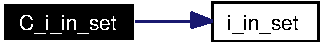
\includegraphics[width=96pt]{Utils_8h_ff0eae9aa0175cd8fe73324707418ce0_cgraph}
\end{center}
\end{figure}
\hypertarget{Utils_8h_12e882779ecd0445c3a0dd9ac85dfeee}{
\index{Utils.h@{Utils.h}!C\_\-kronecker@{C\_\-kronecker}}
\index{C\_\-kronecker@{C\_\-kronecker}!Utils.h@{Utils.h}}
\subsubsection[{C\_\-kronecker}]{\setlength{\rightskip}{0pt plus 5cm}void C\_\-kronecker (const double $\ast$ {\em A}, \/  const int {\em m}, \/  const int {\em n}, \/  const double $\ast$ {\em B}, \/  const int {\em r}, \/  const int {\em s}, \/  double $\ast$ {\em ans})}}
\label{Utils_8h_12e882779ecd0445c3a0dd9ac85dfeee}


Computes the Kronecker product of two matrices\par
 \begin{Desc}
\item[Parameters:]
\begin{description}
\item[{\em A}]matrix \item[{\em m}]nrow(A) \item[{\em n}]ncol(A) \item[{\em B}]matrix \item[{\em r}]nrow(B) \item[{\em s}]ncol(B) \item[{\em ans}]return value; a pointer to a REALSXP-vector of length (mr x ns) \end{description}
\end{Desc}


Definition at line 23 of file Utils.c.

Referenced by C\_\-ExpectCovarLinearStatistic(), and R\_\-kronecker().\hypertarget{Utils_8h_4a31a46e68c52043a6db487de647f774}{
\index{Utils.h@{Utils.h}!C\_\-matprod@{C\_\-matprod}}
\index{C\_\-matprod@{C\_\-matprod}!Utils.h@{Utils.h}}
\subsubsection[{C\_\-matprod}]{\setlength{\rightskip}{0pt plus 5cm}void C\_\-matprod (double $\ast$ {\em x}, \/  int {\em nrx}, \/  int {\em ncx}, \/  double $\ast$ {\em y}, \/  int {\em nry}, \/  int {\em ncy}, \/  double $\ast$ {\em z})}}
\label{Utils_8h_4a31a46e68c52043a6db487de647f774}


matrix product x $\ast$\% y \begin{Desc}
\item[Parameters:]
\begin{description}
\item[{\em x}]a matrix \item[{\em nrx}]number of rows of x \item[{\em ncx}]number of cols of x \item[{\em y}]a matrix \item[{\em nry}]number of rows of y \item[{\em ncy}]number of cols of y \item[{\em z}]a matrix of dimension nrx x ncy \end{description}
\end{Desc}


Definition at line 353 of file Utils.c.

Referenced by R\_\-matprod().\hypertarget{Utils_8h_9097078e7e5f9b9e900a49f07b99efff}{
\index{Utils.h@{Utils.h}!C\_\-matprodT@{C\_\-matprodT}}
\index{C\_\-matprodT@{C\_\-matprodT}!Utils.h@{Utils.h}}
\subsubsection[{C\_\-matprodT}]{\setlength{\rightskip}{0pt plus 5cm}void C\_\-matprodT (double $\ast$ {\em x}, \/  int {\em nrx}, \/  int {\em ncx}, \/  double $\ast$ {\em y}, \/  int {\em nry}, \/  int {\em ncy}, \/  double $\ast$ {\em z})}}
\label{Utils_8h_9097078e7e5f9b9e900a49f07b99efff}


matrix product x $\ast$\% t(y) \begin{Desc}
\item[Parameters:]
\begin{description}
\item[{\em x}]a matrix \item[{\em nrx}]number of rows of x \item[{\em ncx}]number of cols of x \item[{\em y}]a matrix \item[{\em nry}]number of rows of y \item[{\em ncy}]number of cols of y \item[{\em z}]a matrix of dimension nrx x ncy \end{description}
\end{Desc}


Definition at line 405 of file Utils.c.

Referenced by R\_\-matprodT().\hypertarget{Utils_8h_5b306a6923d1155e6ce877cf6fa12a42}{
\index{Utils.h@{Utils.h}!C\_\-max@{C\_\-max}}
\index{C\_\-max@{C\_\-max}!Utils.h@{Utils.h}}
\subsubsection[{C\_\-max}]{\setlength{\rightskip}{0pt plus 5cm}double C\_\-max (const double $\ast$ {\em x}, \/  const int {\em n})}}
\label{Utils_8h_5b306a6923d1155e6ce877cf6fa12a42}


the maximum of a double vector \begin{Desc}
\item[Parameters:]
\begin{description}
\item[{\em x}]vector \item[{\em n}]its length \end{description}
\end{Desc}


Definition at line 278 of file Utils.c.

Referenced by C\_\-maxabsTestStatistic(), C\_\-MonteCarlo(), C\_\-Node(), and R\_\-max().\hypertarget{Utils_8h_c0d5c2fe971923d7a1b1869dffabddb1}{
\index{Utils.h@{Utils.h}!C\_\-MPinv@{C\_\-MPinv}}
\index{C\_\-MPinv@{C\_\-MPinv}!Utils.h@{Utils.h}}
\subsubsection[{C\_\-MPinv}]{\setlength{\rightskip}{0pt plus 5cm}void C\_\-MPinv (SEXP {\em x}, \/  double {\em tol}, \/  SEXP {\em svdmem}, \/  SEXP {\em ans})}}
\label{Utils_8h_c0d5c2fe971923d7a1b1869dffabddb1}


Moore-Penrose inverse of a matrix \begin{Desc}
\item[Parameters:]
\begin{description}
\item[{\em x}]matrix \item[{\em tol}]a tolerance bound \item[{\em svdmem}]an object of class `svd\_\-mem' \item[{\em ans}]return value; an object of class `ExpectCovarMPinv' \end{description}
\end{Desc}


Definition at line 185 of file Utils.c.

References CR\_\-svd(), PL2\_\-MPinvSym, PL2\_\-rankSym, PL2\_\-sSym, PL2\_\-uSym, and PL2\_\-vSym.

Referenced by C\_\-LinStatExpCovMPinv(), and R\_\-MPinv().

Here is the call graph for this function:\nopagebreak
\begin{figure}[H]
\begin{center}
\leavevmode
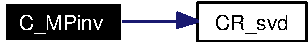
\includegraphics[width=145pt]{Utils_8h_c0d5c2fe971923d7a1b1869dffabddb1_cgraph}
\end{center}
\end{figure}
\hypertarget{Utils_8h_ccce6f00d55276c0a01b30651f1c206c}{
\index{Utils.h@{Utils.h}!C\_\-remove\_\-weights@{C\_\-remove\_\-weights}}
\index{C\_\-remove\_\-weights@{C\_\-remove\_\-weights}!Utils.h@{Utils.h}}
\subsubsection[{C\_\-remove\_\-weights}]{\setlength{\rightskip}{0pt plus 5cm}void C\_\-remove\_\-weights (SEXP {\em subtree})}}
\label{Utils_8h_ccce6f00d55276c0a01b30651f1c206c}


Remove weights vector from each node of a tree (in order to save memory) $\backslash$$\ast$param subtree a tree 

Definition at line 702 of file Utils.c.

References C\_\-remove\_\-weights(), S3\_\-WEIGHTS, S3get\_\-leftnode(), S3get\_\-nodeterminal(), and S3get\_\-rightnode().

Referenced by C\_\-remove\_\-weights(), R\_\-Ensemble(), and R\_\-remove\_\-weights().

Here is the call graph for this function:\nopagebreak
\begin{figure}[H]
\begin{center}
\leavevmode
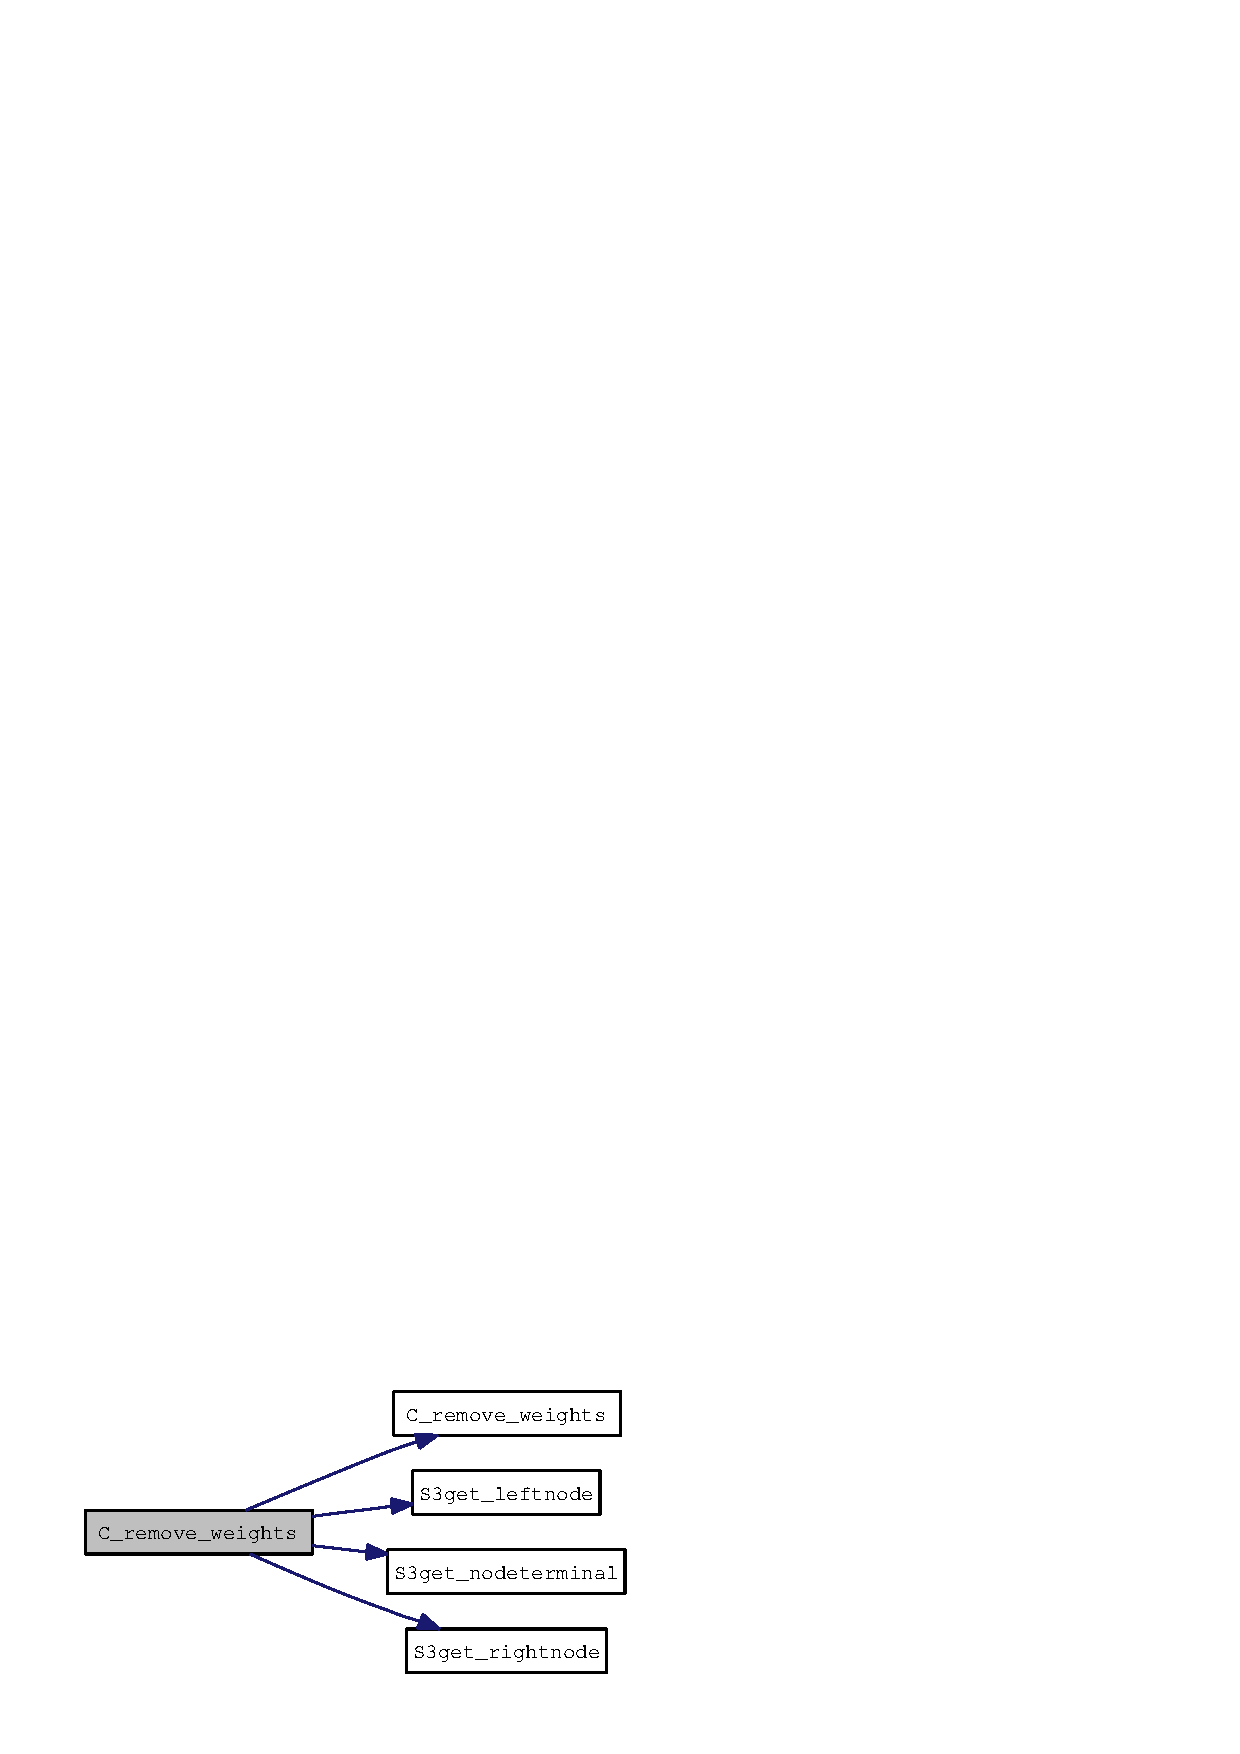
\includegraphics[width=209pt]{Utils_8h_ccce6f00d55276c0a01b30651f1c206c_cgraph}
\end{center}
\end{figure}
\hypertarget{Utils_8h_f7c710920d1496d23fdabad9b1d0e18c}{
\index{Utils.h@{Utils.h}!C\_\-SampleNoReplace@{C\_\-SampleNoReplace}}
\index{C\_\-SampleNoReplace@{C\_\-SampleNoReplace}!Utils.h@{Utils.h}}
\subsubsection[{C\_\-SampleNoReplace}]{\setlength{\rightskip}{0pt plus 5cm}void C\_\-SampleNoReplace (int $\ast$ {\em x}, \/  int {\em m}, \/  int {\em k}, \/  int $\ast$ {\em ans})}}
\label{Utils_8h_f7c710920d1496d23fdabad9b1d0e18c}


compute a permutation of a (random subset of) 0:(m-1) \begin{Desc}
\item[Parameters:]
\begin{description}
\item[{\em x}]an integer vector of length m \item[{\em m}]integer \item[{\em k}]integer \item[{\em ans}]an integer vector of length k \end{description}
\end{Desc}


Definition at line 453 of file Utils.c.

Referenced by C\_\-GlobalTest(), C\_\-MonteCarlo(), R\_\-permute(), and R\_\-rsubset().\hypertarget{Utils_8h_88c1a807c7856d57d07d10027d588602}{
\index{Utils.h@{Utils.h}!C\_\-SampleSplitting@{C\_\-SampleSplitting}}
\index{C\_\-SampleSplitting@{C\_\-SampleSplitting}!Utils.h@{Utils.h}}
\subsubsection[{C\_\-SampleSplitting}]{\setlength{\rightskip}{0pt plus 5cm}void C\_\-SampleSplitting (int {\em n}, \/  double $\ast$ {\em prob}, \/  int $\ast$ {\em weights}, \/  int {\em k})}}
\label{Utils_8h_88c1a807c7856d57d07d10027d588602}




Definition at line 679 of file Utils.c.

References C\_\-ProbSampleNoReplace().

Referenced by R\_\-Ensemble().

Here is the call graph for this function:\nopagebreak
\begin{figure}[H]
\begin{center}
\leavevmode
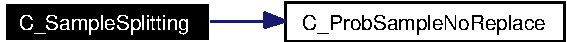
\includegraphics[width=153pt]{Utils_8h_88c1a807c7856d57d07d10027d588602_cgraph}
\end{center}
\end{figure}
\hypertarget{Utils_8h_f9716d8427688ac52d3dd254337316b1}{
\index{Utils.h@{Utils.h}!C\_\-tempweights@{C\_\-tempweights}}
\index{C\_\-tempweights@{C\_\-tempweights}!Utils.h@{Utils.h}}
\subsubsection[{C\_\-tempweights}]{\setlength{\rightskip}{0pt plus 5cm}double$\ast$ C\_\-tempweights (int {\em j}, \/  SEXP {\em weights}, \/  SEXP {\em fitmem}, \/  SEXP {\em inputs})}}
\label{Utils_8h_f9716d8427688ac52d3dd254337316b1}




Definition at line 718 of file Utils.c.

References get\_\-missings(), and get\_\-weights().

Referenced by C\_\-GlobalTest(), C\_\-Node(), and C\_\-surrogates().

Here is the call graph for this function:\nopagebreak
\begin{figure}[H]
\begin{center}
\leavevmode
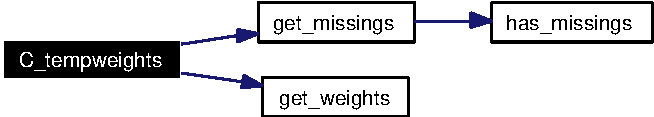
\includegraphics[width=175pt]{Utils_8h_f9716d8427688ac52d3dd254337316b1_cgraph}
\end{center}
\end{figure}
\hypertarget{Utils_8h_2a701345082320c18e49d8e7e8150d64}{
\index{Utils.h@{Utils.h}!C\_\-whichmax@{C\_\-whichmax}}
\index{C\_\-whichmax@{C\_\-whichmax}!Utils.h@{Utils.h}}
\subsubsection[{C\_\-whichmax}]{\setlength{\rightskip}{0pt plus 5cm}int C\_\-whichmax (double $\ast$ {\em pvalue}, \/  double $\ast$ {\em teststat}, \/  int {\em ninputs})}}
\label{Utils_8h_2a701345082320c18e49d8e7e8150d64}




Definition at line 583 of file Utils.c.

Referenced by C\_\-Node(), and R\_\-whichmax().\hypertarget{Utils_8h_ae969040bb060d2874fd969e20675bbb}{
\index{Utils.h@{Utils.h}!i\_\-in\_\-set@{i\_\-in\_\-set}}
\index{i\_\-in\_\-set@{i\_\-in\_\-set}!Utils.h@{Utils.h}}
\subsubsection[{i\_\-in\_\-set}]{\setlength{\rightskip}{0pt plus 5cm}int i\_\-in\_\-set (int {\em i}, \/  int $\ast$ {\em iset}, \/  int {\em p})}}
\label{Utils_8h_ae969040bb060d2874fd969e20675bbb}


determine if i is element of the integer vector set \begin{Desc}
\item[Parameters:]
\begin{description}
\item[{\em i}]an integer \item[{\em iset}]a pointer to an integer vector \item[{\em p}]length(iset) \end{description}
\end{Desc}


Definition at line 549 of file Utils.c.

Referenced by C\_\-i\_\-in\_\-set(), and C\_\-splitnode().\hypertarget{Utils_8h_572286b2fd0bd9993473cfd0c6b165c0}{
\index{Utils.h@{Utils.h}!La\_\-svd@{La\_\-svd}}
\index{La\_\-svd@{La\_\-svd}!Utils.h@{Utils.h}}
\subsubsection[{La\_\-svd}]{\setlength{\rightskip}{0pt plus 5cm}SEXP La\_\-svd (SEXP {\em jobu}, \/  SEXP {\em jobv}, \/  SEXP {\em x}, \/  SEXP {\em s}, \/  SEXP {\em u}, \/  SEXP {\em v}, \/  SEXP {\em method})}}
\label{Utils_8h_572286b2fd0bd9993473cfd0c6b165c0}


\hypertarget{Utils_8h_d91bea0afb4613aab593f6311318a63c}{
\index{Utils.h@{Utils.h}!ncol@{ncol}}
\index{ncol@{ncol}!Utils.h@{Utils.h}}
\subsubsection[{ncol}]{\setlength{\rightskip}{0pt plus 5cm}int ncol (SEXP {\em y})}}
\label{Utils_8h_d91bea0afb4613aab593f6311318a63c}




Definition at line 575 of file Utils.c.

Referenced by C\_\-GlobalTest(), C\_\-IndependenceTest(), C\_\-MonteCarlo(), C\_\-Node(), C\_\-splitnode(), R\_\-Ensemble(), R\_\-ExpectCovarInfluence(), R\_\-ExpectCovarLinearStatistic(), R\_\-LinearStatistic(), R\_\-matprod(), R\_\-matprodT(), R\_\-MPinv(), R\_\-Node(), R\_\-PermutedLinearStatistic(), R\_\-split(), R\_\-splitcategorical(), and R\_\-TreeGrow().\hypertarget{Utils_8h_eeb672a71c45ead28b7b354414f2427a}{
\index{Utils.h@{Utils.h}!nrow@{nrow}}
\index{nrow@{nrow}!Utils.h@{Utils.h}}
\subsubsection[{nrow}]{\setlength{\rightskip}{0pt plus 5cm}int nrow (SEXP {\em x})}}
\label{Utils_8h_eeb672a71c45ead28b7b354414f2427a}




Definition at line 571 of file Utils.c.

Referenced by C\_\-GlobalTest(), C\_\-IndependenceTest(), CR\_\-svd(), R\_\-ExpectCovarInfluence(), R\_\-ExpectCovarLinearStatistic(), R\_\-LinearStatistic(), R\_\-matprod(), R\_\-matprodT(), R\_\-maxabsConditionalPvalue(), R\_\-MPinv(), R\_\-PermutedLinearStatistic(), R\_\-split(), and R\_\-splitcategorical().